\documentclass[tikz,border=2mm]{standalone}
\usepackage{tikz}

\begin{document}

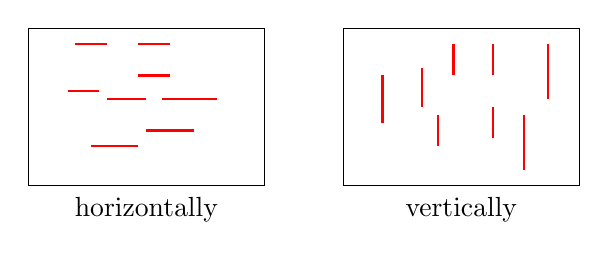
\begin{tikzpicture}
    \begin{scope}[shift={(0,0)}] % move to the right
    \draw (0,0) rectangle (3,2);
    \draw[red, thick] (1.5, 1.1) -- (1, 1.1);
    \draw[red, thick] (0.9, 1.2) -- (0.5, 1.2);
    \draw[red, thick] (1.4, 1.4) -- (1.8, 1.4);
    \draw[red, thick] (1.4, 1.8) -- (1.8, 1.8);
    \draw[red, thick] (0.6, 1.8) -- (1, 1.8);
    \draw[red, thick] (0.8, 0.5) -- (1.4, 0.5);
    \draw[red, thick] (1.7, 1.1) -- (2.4, 1.1);
    \draw[red, thick] (1.5, 0.7) -- (2.1, 0.7);
    % Label below
    \node at (1.5,-0.3) {horizontally};
  \end{scope}
  % First rectangle and red lines (vertical)
  \begin{scope}[shift={(4,0)}]
    \draw (0,0) rectangle (3,2);
    \draw[red, thick] (1,1.5) -- (1,1);
    \draw[red, thick] (1.2, 0.9) -- (1.2, 0.5);
    \draw[red, thick] (1.4, 1.4) -- (1.4, 1.8);
    \draw[red, thick] (1.9, 1.4) -- (1.9, 1.8);
    \draw[red, thick] (1.9, 0.6) -- (1.9, 1);
    \draw[red, thick] (0.5, 0.8) -- (0.5, 1.4);
    \draw[red, thick] (2.3, 0.2) -- (2.3, 0.9 );
    \draw[red, thick] (2.6, 1.1) -- (2.6, 1.8 );
    % Label below
    \node at (1.5,-0.3) {vertically};
  \end{scope}

  % Second rectangle and red lines (horizontal)

\end{tikzpicture}

\end{document}